\documentclass[12pt,a4paper]{article}
\usepackage{amsmath,amscd,amsbsy,amssymb,latexsym,url,bm,amsthm}
\usepackage{epsfig,graphicx,subfigure}
\usepackage{enumitem,balance}
\usepackage{wrapfig}
\usepackage{mathrsfs,euscript}
\usepackage[usenames]{xcolor}
\usepackage{hyperref}
\usepackage[vlined,ruled,linesnumbered]{algorithm2e}
\usepackage{graphicx} %插入图片的宏包
\usepackage{float} %设置图片浮动位置的宏包
\usepackage{subfigure} %插入多图时用子图显示的宏包
\usepackage{listings}
\hypersetup{colorlinks=true,linkcolor=black}

%\usepackage{listings} % 插入程序的包
%\begin{document}
%\lstset{breaklines=true}
%\lstinputlisting[language=c++]{File.cpp}
%\end{document}


\newtheorem{theorem}{Theorem}
\newtheorem{lemma}[theorem]{Lemma}
\newtheorem{proposition}[theorem]{Proposition}
\newtheorem{corollary}[theorem]{Corollary}
\newtheorem{exercise}{Exercise}
\newtheorem*{solution}{Solution}
\newtheorem{definition}{Definition}
\theoremstyle{definition}

\renewcommand{\thefootnote}{\fnsymbol{footnote}}

\newcommand{\postscript}[2]
 {\setlength{\epsfxsize}{#2\hsize}
  \centerline{\epsfbox{#1}}}

\renewcommand{\baselinestretch}{1.0}

\setlength{\oddsidemargin}{-0.365in}
\setlength{\evensidemargin}{-0.365in}
\setlength{\topmargin}{-0.3in}
\setlength{\headheight}{0in}
\setlength{\headsep}{0in}
\setlength{\textheight}{10.1in}
\setlength{\textwidth}{7in}
\makeatletter \renewenvironment{proof}[1][Proof] {\par\pushQED{\qed}\normalfont\topsep6\p@\@plus6\p@\relax\trivlist\item[\hskip\labelsep\bfseries#1\@addpunct{.}]\ignorespaces}{\popQED\endtrivlist\@endpefalse} \makeatother
\makeatletter
\renewenvironment{solution}[1][Solution] {\par\pushQED{\qed}\normalfont\topsep6\p@\@plus6\p@\relax\trivlist\item[\hskip\labelsep\bfseries#1\@addpunct{.}]\ignorespaces}{\popQED\endtrivlist\@endpefalse} \makeatother

\begin{document}
\noindent

%========================================================================
\noindent\framebox[\linewidth]{\shortstack[c]{
\Large{\textbf{Lab02-Divide and Conquer}}\vspace{1mm}\\
CS214-Algorithm and Complexity, Xiaofeng Gao, Spring 2021.}}
\begin{center}
\footnotesize{\color{red}$*$ If there is any problem, please contact TA Haolin Zhou. }

\footnotesize{\color{blue}$*$ Name:Zirui Liu \quad Student ID:519021910343 \quad Email: L.prime@sjtu.edu.cn}
\end{center}

\begin{enumerate}
\item
    \textit{Recurrence examples.} Give asymptotic upper and lower bounds for $T(n)$ in each of the following recurrences. Assume that $T(n)$ is constant for sufficiently small $n$. Make your bounds as tight as possible.
\begin{enumerate}
	\item $T(n)=4 T(n / 3)+n \log n$
	\item $T(n)=4 T(n / 2)+n^{2} \sqrt{n}$
	\item $T(n)=T(n-1)+n$	
	\item $T(n)=2T(\lfloor \sqrt n\rfloor)+\log n$
\end{enumerate}
\begin{solution}
	%response...
	we apply the following conclusion: Let $f(n)$ be $n \log n$, if $f(n)=O\left(n^{\log_ b a}*\lg^k n \right)$ then $T(n)=O\left(n^{\log_ b a}*\lg^{k+1} n \right)$. So $T(n)$ for $(a)$ is 

	(1) for $T(n)=4 T(n / 3)+n \log n$, $a=4$, $b=3$, $ 1 < d < \log_3 4 $, since $n\log n < n^{\frac{4}{3}}$, so applying the Master Theorem, we can conclude that $T(n)=O(n^{\log_ 3 4})$.
	
	(2) for $T(n)=4 T(n / 2)+n^{2} \sqrt{n}$ , we can simply apply the Master Theorem, $a=4$, $b=2$, $d=2.5$, so $T(n)=O(n^{2.5})$.
	
	(3) for $T(n)=T(n-1)+n$, by simply applying recursion, we can know that $T\left(n\right)=n!$
	
	(4) for $T(n)=2T(\lfloor \sqrt n\rfloor)+\log n$ if we do some simple algorithm transformations, let $m=\log n$, then we have $T\left(2^m\right)=2T\left(2^{\frac{m}{2}}\right)+m$, then we let $S\left(m\right)=T\left(2^m\right)$, so we got $S\left(m\right)=2S\left(\frac{m}{2}\right)+m$, so $S\left(m\right)=O\left(m\lg m\right)$. Then we take this equation back to its former relation, we can conclude that $T\left(n\right)=O\left(\lg n \lg\lg n\right)$. 
	
	
\end{solution}
\item
\textit{Divide-and-conquer.} Given an integer array $A[1..n]$ and two integers $lower \le upper$, design an algorithm using \textbf{divide-and-conquer} method to count the number of ranges $(i,j)$ ($1 \leq i \leq j \leq n$) satisfying
$$
    lower \leq \sum_{k=i}^{j}{A[k]} \leq upper.
$$
\textbf{Example:}

Given $A = [1,-1,2]$, $lower = 1$, $upper = 2$, return 4.

The resulting four ranges are $(1,1)$, $(3,3)$, $(2,3)$ and $(1,3)$.

\begin{enumerate}
\item
Complete the implementation in the provided C/C++ source code {\color{blue}(The source code \emph{Code-Range.cpp} is attached on the course webpage)}.

\begin{solution}
Please check out in the appendix.
\end{solution}

\item
Write a recurrence for the running time of the algorithm and solve it by recurrence tree {\color{blue}(You can modify the figure sources \emph{Fig-RecurrenceTree.vsdx} or \emph{Fig-RecurrenceTree.pptx} to illustrate your derivation)}.

%\begin{figure}[H] %H为当前位置,!htb为忽略美学标准,htbp为浮动图形
%\centering %图片居中
%\includegraphics[width=0.4\textwidth]{figures/relationship.png} %%插入图片,[]中设置图片大小,{}中是图片文件名
%\caption{Diagram of the relationship between the elements} %%最终文档中希望显示的图片标题
%\label{fig1} %用于文内引用的标签
%\end{figure}

\begin{figure}[the]
    \centering
    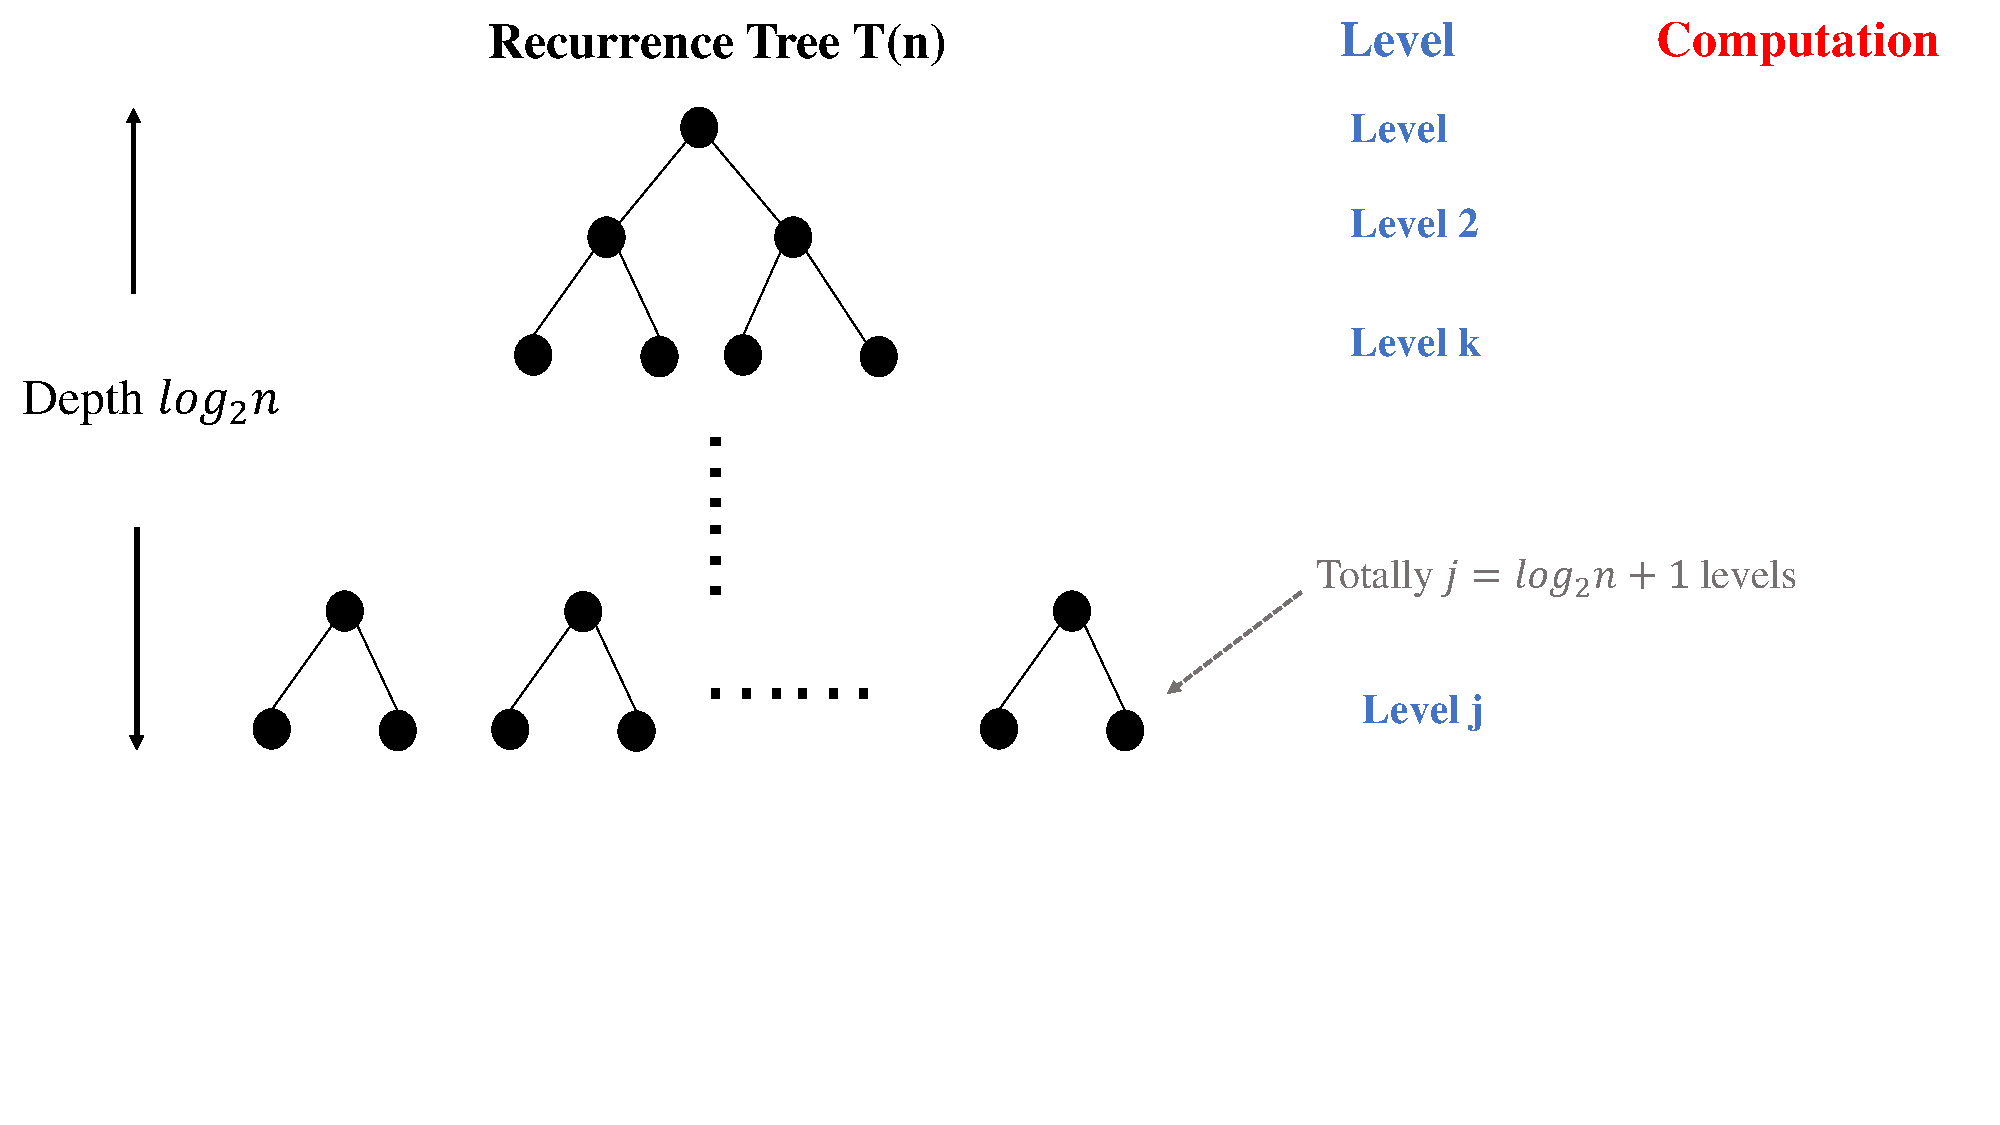
\includegraphics[width=0.8\textwidth]{Fig-RecurrenceTree2.pdf}
    \caption{RecurrenceTree}\label{Fig-Transposition}
\end{figure}

\begin{solution}
% for 2(b) 
Since the algorithm has time complexity of $T\left(n\right)=2T\left(\frac{n}{2}\right)+n\log n$, We can conclude from the recursive tree that in the j-th level, there exists a time complexity of $2^{j-1}*O\left(\frac{n}{2^{j-1}}*\log \frac{n}{2^{j-1}}\right)$, so we calculate the sum of this equation, and we ignore the constant items of the function, we get $\left(\log_2 n +1\right)*n*\log n$, that is the time complexity of $T\left(n\right)=n\log^2 n$. 
\end{solution}


\item
Can we use the Master Theorem to solve the recurrence above? Please explain your answer.
\end{enumerate}
\begin{solution}
%response...
We can't apply the original edition of Master Theorem, but we can apply a modified version. We apply the following conclusion: Let $f(n)$ be $n \log n$, if $f(n)=O\left(n^{\log_ b a}*\lg^k n \right)$ then $T(n)=O\left(n^{\log_ b a}*\lg^{k+1} n \right)$. So $T(n)$ for this situation is $T\left(n\right)=O\left(n\log^2 n\right)$.  
\end{solution}
\item
\textit{Transposition Sorting Network.} A comparison network is a \textbf{transposition network}  if each comparator connects adjacent lines, as in the network in Fig.~\ref{Fig-Transposition}.

\begin{figure}[htbp]
    \centering
    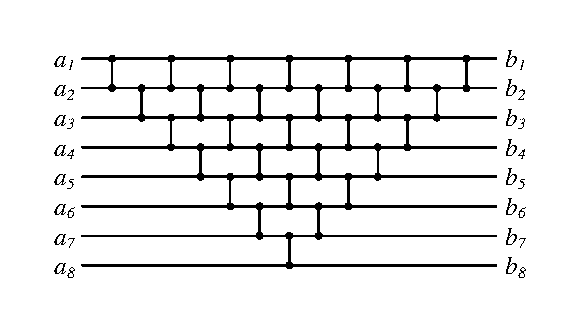
\includegraphics[width=0.4\textwidth]{Fig-Transposition.pdf}
    \caption{A Transposition Network Example}\label{Fig-Transposition}
\end{figure}

\begin{enumerate}
\item Prove that a transposition network with $n$ inputs is a sorting network if and only if it sorts the sequence $\langle n, n-1, \cdots, 1 \rangle$. {\color{blue}(Hint: Use an induction argument analogous to the \emph{Domain Conversion Lemma}.)}
\item {\color{red}{(Optional Sub-question with Bonus)}} Given any $n \in \mathbb{N}$, write a program using Tkinter in Python to draw a figure similar to Fig.~\ref{Fig-Transposition} with $n$ input wires.
\end{enumerate}
\end{enumerate}
\begin{solution}
%response...
Consider an input  $\langle n, n-1, \cdots, 1 \rangle$ to a transposition network and the state of the network
after the $k$-th comparator. We denote the data held by line after the $k$-th comparator by  $i_{x k}$. We use induction over the comparators in order.
For a base case, consider the network before any comparators. For any $i$ and $j$ with  
 $i<j$, $i_D,0 > j_D,0$
because the input is descending. Thus, we make no claim about any of the  $i_X,0 $.
Assume that the claim holds after the $k-1$-th comparator. Consider the $k$-th comparator. Because we
have a transposition network, we compare two adjacent lines $i$ and $i+1$ . We need to show that the
claim holds (for all pairs) of lines after the $k$-th comparator. That is, consider any two lines $a$ and $b$ with
 $1\leq a<b\leq r$. Suppose that $a_D,k < b_D,k $. Then we need to show that $a_X,k < b_X,k $. 
 
 To be honest, I myself can't proof this and I think it is too difficult. I thought it for many hours and I haven't figured it out. But I found the original answer in  \cite{ref1}.

\end{solution}
%========================================================================
\newpage

\begin{appendices}
\section{First appendix}
\textcolor[rgb]{0.98,0.00,0.00}{\textbf{Input C++ source1:}}
\lstinputlisting[language=c++]{./Code-Range.cpp}

%\t

%\section{Second appendix}

%\textcolor[rgb]{0.98,0.00,0.00}{\textbf{Input python source2:}}
%\lstinputlisting[language=python]{./code/fire_data.py}

\end{appendices}

\begin{thebibliography}{99}
    \bibitem{ref1} https://ocw.mit.edu/courses/electrical-engineering-and-computer-science/6-896-theory-of-parallel-hardware-sma-5511-spring-2004/assignments/sol6.pdf


\end{thebibliography}


\end{document}
